\chapter{Results and Discussion}\label{chapter:Results}
This chapter presents and analyses the results obtained from applying the \ac{ITM} on seismic waves.
We begin by examining the travelling planar wave before addressing point sources. 
As a starting point, the time-reversal is analysed in an acoustic media with an initial condition
as a travelling planar P-Wave in section \ref{sec:acoustictravelling}. The second part deals with the time-reversal of a velocity impulse point source in an acoustic medium. The third part deals with the time-reversal
of a velocity impulse point source in an elastic medium with refocusing of both P- and S-waves together and separately in sections \ref{sec:acousticITM} to \ref{sec:elasticITMswave}. 
In sections \ref{sec:pressureimpulse} and \ref{sec:doublecouple}, we demostrate the application of \ac{ITM} in reversing waves generated by moment tensors. In all the cases, we check if the refocused wave will converge to the location of the source with the same speed as the original wave. We analyse all cases with a homogenous medium to deliver on a sound proof of concept of the \ac{ITM} being useful to refocus different kind of waves. We used a modification
of our benchmark test problem, WP2-LOH1 to show refocusing in realistic media.\\
To wrap up, we perform a convergence test to check the correctness of our \ac{ITM} implementation with the analytical solutions derived in section \ref{section:3DITMAcoustic}.

\section{Time-reversal of a travelling planar P-wave} \label{sec:acoustictravelling}
The acoustic case is a simplification of propagation in an elastic medium. The second Lam\'{e} parameter $\mu$ is set to zero. The medium is characterized by
\begin{equation}
    \rho = 4, \quad \mu = 0, \quad \lambda = 1 .
\end{equation}

The propagation speed of the P-wave in this case is given by
\begin{equation}
    v_p = \sqrt{\frac{\lambda + 2 \mu}{\rho}} = \sqrt{\frac{1}{4}} = \frac{1}{2} .
\end{equation}

We impose an initial condition such that there is a P-Wave travelling towards the negative x-axis. The details on how the initial conditions are set up to ensure a left going P-wave is discussed in
\href{https://seissol.readthedocs.io/en/latest/initial-condition.html#travelling-wave}{Travelling Wave: SeisSol}\footnote{\href{https://seissol.readthedocs.io/en/latest/initial-condition.html\#travelling-wave}{https://seissol.readthedocs.io/en/latest/initial-condition.html\#travelling-wave}}. We impose a P-Wave with a wavelength of 
$\lambda = 1.0$. This gives us a timeperiod of $T=2.0$. We choose a cubic computational domain of [-1, 1] in all three directions with periodic boundary conditions with the triangular mesh shown in figure \ref{fig:acoustic_mesh} which contains
163840 triangular elements. 

\begin{figure}[htpb]
    \centering
    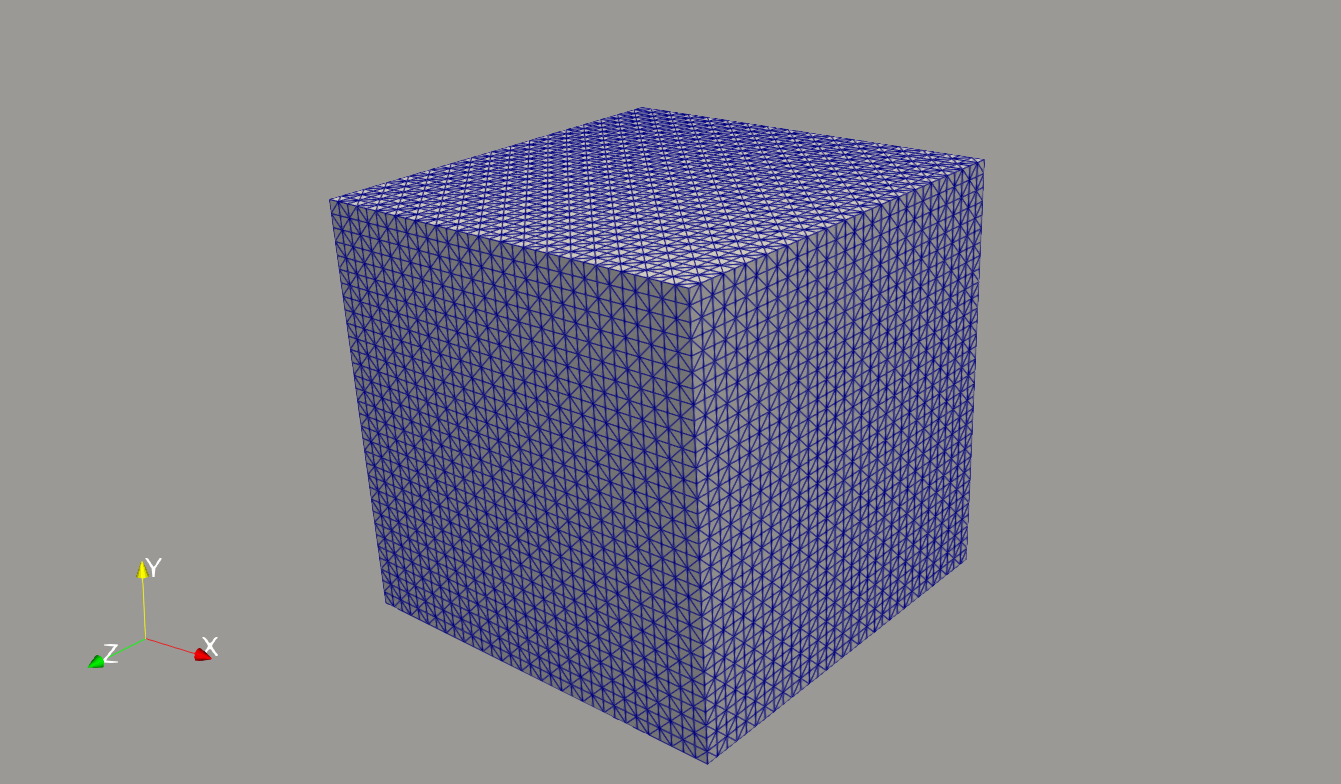
\includegraphics[width=0.85\linewidth]{figures/mesh_cube.png}
    \caption{Mesh used for the simulation of a travelling planar wave in acoustic medium with \ac{ITM}}
    \label{fig:acoustic_mesh}
\end{figure}
\par We start our initial travelling wave at the origin and our wave travels to the boundary in $t = \frac{1}{2}$. We start our \ac{ITM} at $t=2$ such that the reversed wave will travel back to the origin at $t=4.0$ to meet the
forward going wave. 

\begin{figure}[htpb]
    \centering
    \begin{subfigure}[b]{0.495\textwidth}
        \centering
        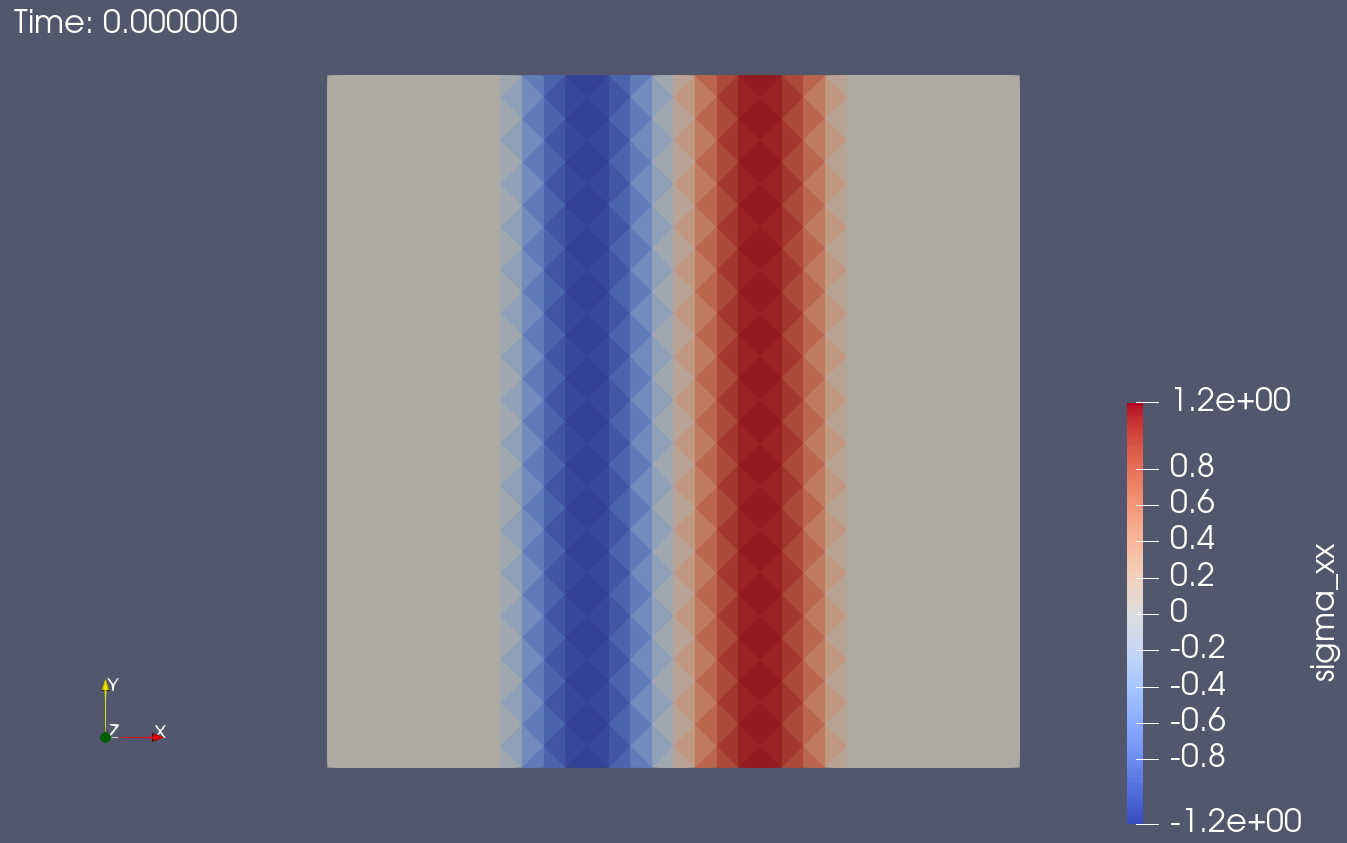
\includegraphics[width=1.0\textwidth]{figures/travellingwave_t0.png}
        \caption{t=0} 
    \end{subfigure}
    \vskip\baselineskip
    \begin{subfigure}[b]{0.495\textwidth}   
        \centering 
        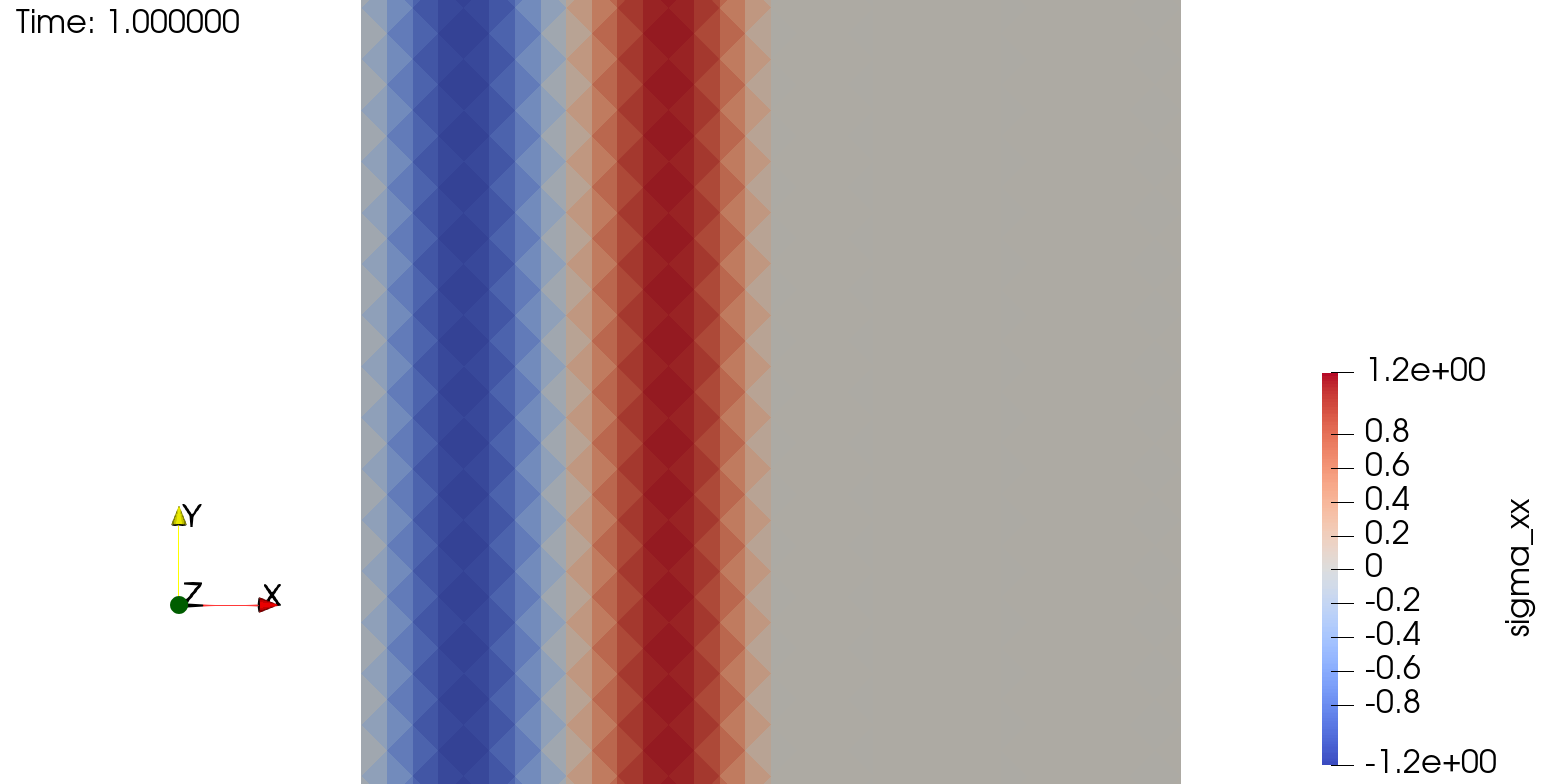
\includegraphics[width=1.0\textwidth]{figures/travellingwave_t1.png}
        \caption{t=1.0}
    \end{subfigure}
    \hfill
    \begin{subfigure}[b]{0.495\textwidth}   
        \centering 
        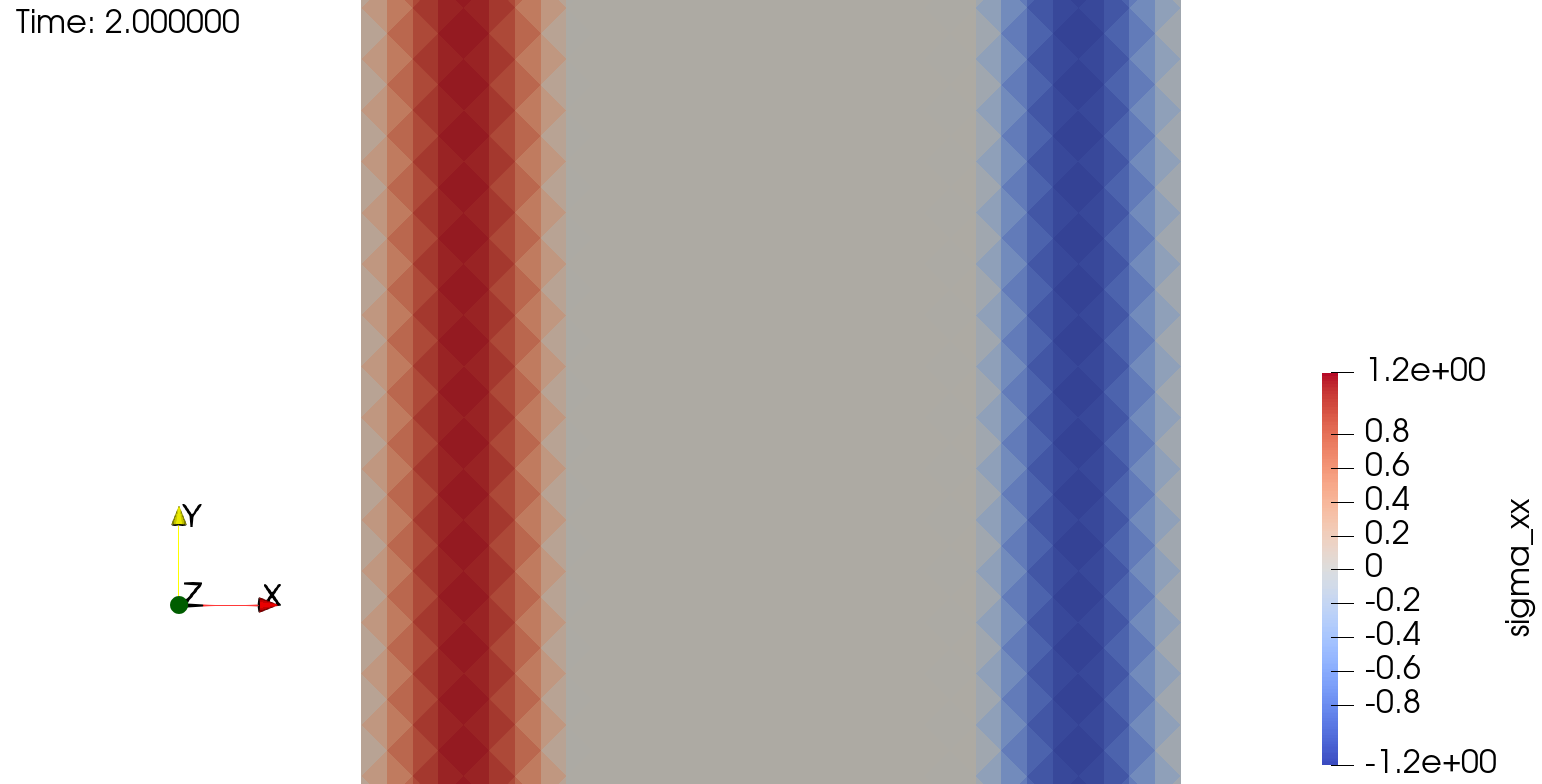
\includegraphics[width=1.0\textwidth]{figures/travellingwave_t2.png}
        \caption{t=2.0}
    \end{subfigure}
    \vskip\baselineskip
    \begin{subfigure}[b]{0.495\textwidth}   
        \centering 
        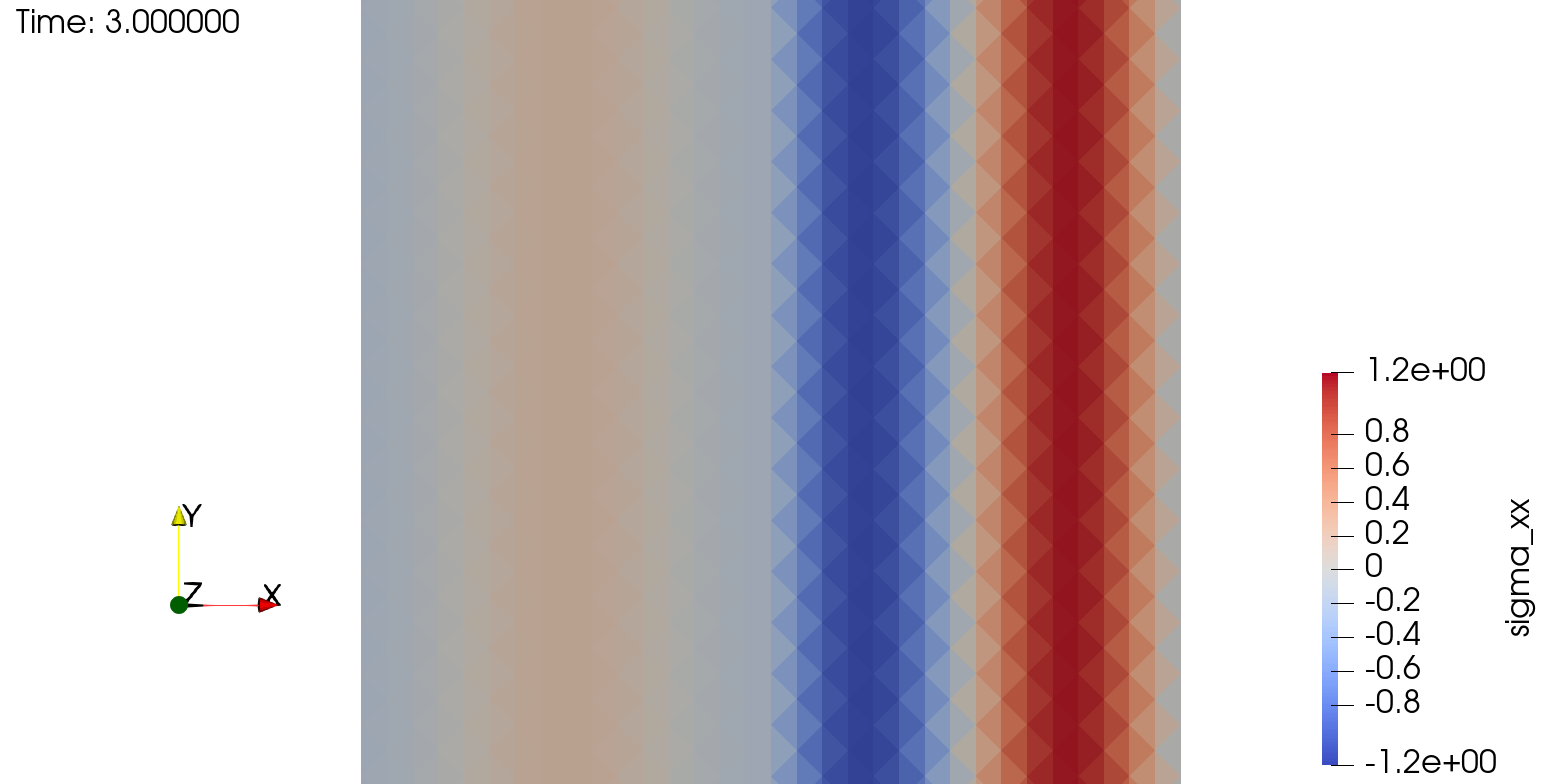
\includegraphics[width=1.0\textwidth]{figures/travellingwave_t3.png}
        \caption{{t=3.0}}
    \end{subfigure}
    \hfill
    \begin{subfigure}[b]{0.495\textwidth}   
        \centering 
        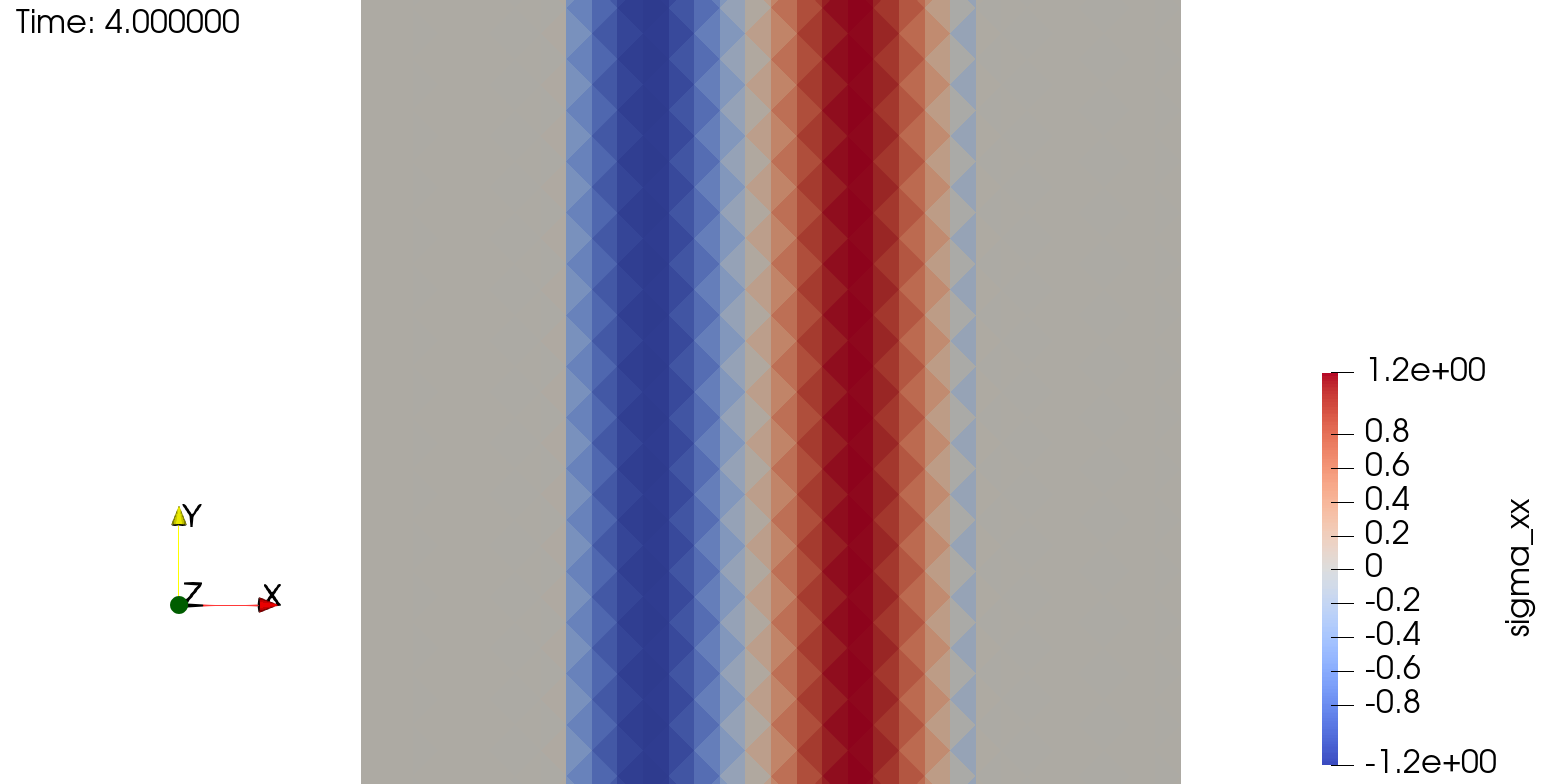
\includegraphics[width=1.0\textwidth]{figures/travellingwave_t4.png}
        \caption{{t=4.0}}
    \end{subfigure}
    \caption{\ac{ITM} applied on a travelling planar wave in an acoustic media.}
    \label{fig:acoustic_travellingwave}
\end{figure}

Figure \ref{fig:acoustic_travellingwave} shows the evolution of the wavefield in time. We notice that there is a reflection of the forward going wave and it meets the forward going wave at the origin at $t=4.0$. This is a proof of concept that the \ac{ITM} can be used to refocus waves in an acoustic media. 

To observe the refocusing in a clearer way, we choose a slice perpendicular to the $z$-axis at the origin and plot the wavefield in terms of $u$-velocity along the $x$-axis
at different times in figure \ref{fig:space-timeplot-travelling}. We can see that at $t=2.0$, there is a reflected component along with the forward component. At $t=3.0$, i.e., half the time-period after
the application of the \ac{ITM}, the reflected component interacts with the forward wave for the first time. This shows that in half the time-period, the reflected wave travelled half the wave length interacting
with the forward travelling wave. At $t=4.0$, the reflected wave has travelled the entire wave length and is refocused at the origin. 

\begin{figure}[htpb]
    \centering
    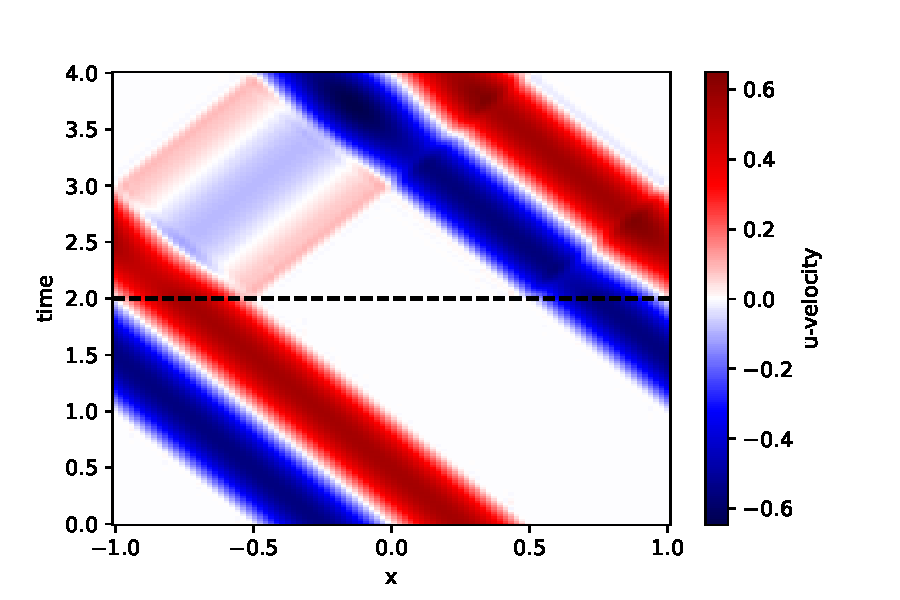
\includegraphics[width=0.75\linewidth]{figures/space-time-plot-travelling.pdf}
    \caption{Space-time plot for Acoustic Travelling Wave with \ac{ITM}. We take a slice perpendicular to the $z$-axis at the origin and plot the $u$-velocity along the $x$-axis at different times.}
    \label{fig:space-timeplot-travelling}
\end{figure}

\section{Time-reversal of wave created by a velocity impulse point source in acoustic media} \label{sec:acousticITM}

We now consider a velocity impulse point source in an acoustic medium. We pick the Lam\'{e} parameter $\lambda$, density $\rho$ 
from the half-space of the benchmark case WP2-LOH1\footnote[1]{https://seissol.readthedocs.io/en/latest/pointsource.html} to make it a homogenous acoustic medium. 
The medium is characterized by
\begin{align}
    \begin{split}
        \rho &=    2700.0 ,\\
        \mu &=     0.0 ,\\
        \lambda &= 3.24038016 \cdot 10^{10} .
    \end{split}
\end{align}

This makes the velocity of the P-wave to be
\begin{equation}
    v_p = \sqrt{\frac{3.24038016 \cdot 10^{10}}{2700}} \approx 3464 .
\end{equation}

We choose a computational domain of $\left[-26000,32000\right] \times \left[-26000,32000\right] \times \left[0,34000\right]$ and a simulation time of $t=10.0$ with \ac{ITM} applied at $t=5.0$ 
such that the originating waves do not reflect back from the boundaries at the $x$- and $y$-axis ensuring that
reflections due to \ac{ITM} are clearly noticeable. Our velocity impulse source is at $\left(3000,3000,17000\right)$, the center of the domain. 
We have used an unstructured tetrahedral mesh with around 1.4 million elements. We have used more refinement in the region close to the source to capture the steep gradients as in figure \ref{fig:mesh-loh1}.

\begin{figure}[htpb]
    \centering
    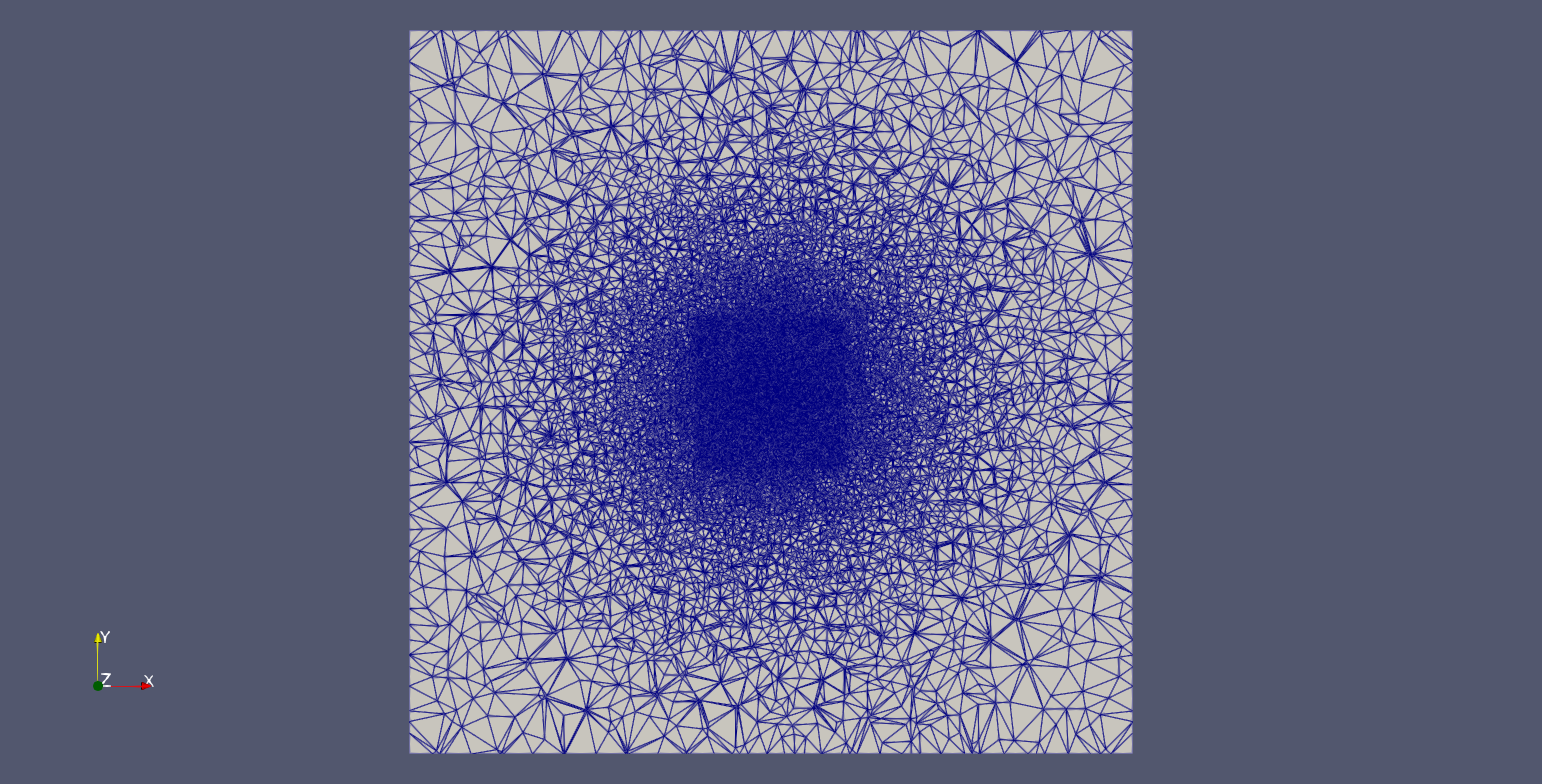
\includegraphics[width=\linewidth]{figures/mesh_loh1.png}
    \caption{Example mesh for simulations with a point source acting as a velocity pulse. We have a finer mesh near the source and a coarser mesh away from the source.}
    \label{fig:mesh-loh1}
\end{figure}

The source term is given as 
\begin{align}
    \begin{split}
        \dot{S} = \frac{1}{T^2} t e^{-\frac{t}{T}} , \\
        S_i = \dot{S} \times C_i ,
    \end{split}
    \label{eq:source}
\end{align}
where T is a constant to decide the duration of the source approximately. This source is then applied to equations 7 to 9 in equation \ref{eq:setofequations} as per the direction
$i$. $i$ is the direction of the source. $i=7$ is a source applied in $x$-direction,
$i=8$ is a source applied in $y$-direction and $i=9$ is a source applied in $z$-direction.

We choose T=0.1 and the source to be in the $z$-direction with $C_7 = 0, C_8 = 0, C_9 = 1.2 \cdot 10^{16}$. With this, our source looks like in figure \ref{fig:source}

\begin{figure}[htpb]
    \centering
    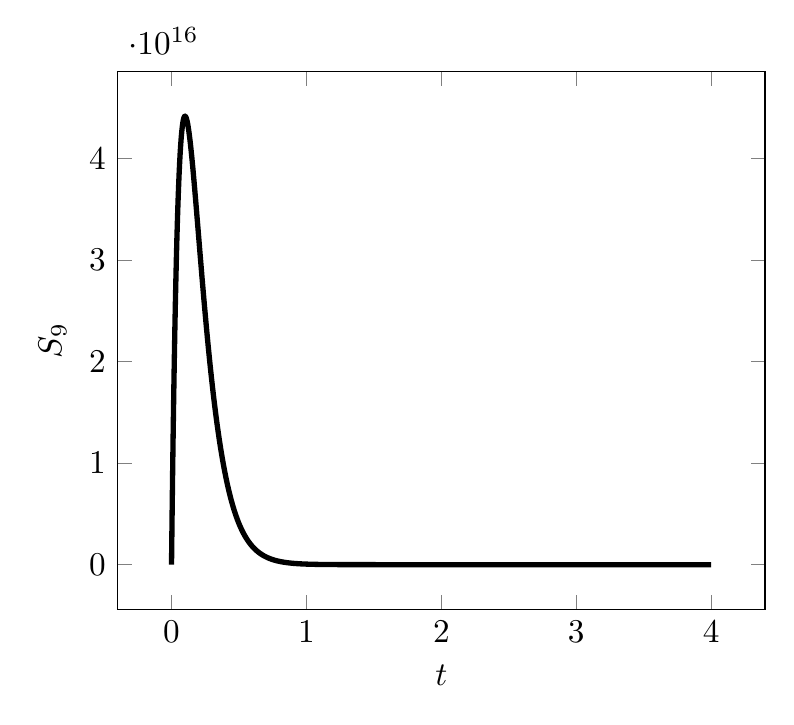
\begin{tikzpicture}[scale=1.2]
        \begin{axis}[
            ylabel = $S_9$,
            xlabel = $t$]
            \addplot[domain=0:4, samples=1001, black, ultra thick]{1.2e16 * x*exp(-x/0.1)/(0.1*0.1)};
        \end{axis}
    \end{tikzpicture}
    \caption{Source term used for velocity impulse point source applied to $z$-velocity}
    \label{fig:source}
\end{figure}

We pick a slice at $\left(3000,3000,20000\right)$, i.e., 3000 away from the source location in $z$-direction.
We plot the $u$-velocities along the $x$-axis at different times on this slice. With this setup and velocity impulse, we see that the velocity in $x$-direction
looks like in figure \ref{fig:space-timeplot-acousticnoITM}.
\begin{figure}[htpb]
    \centering
    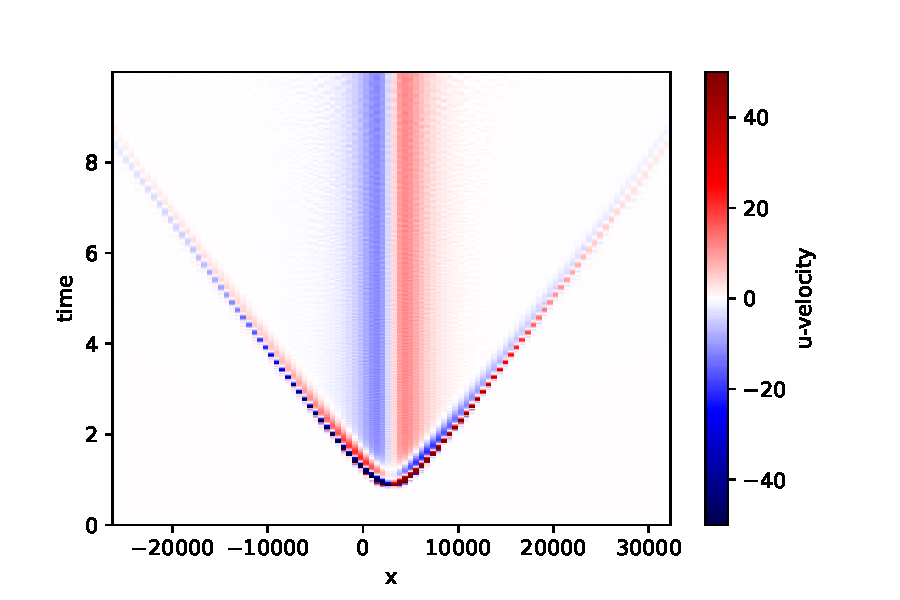
\includegraphics[width=0.9\linewidth]{figures/Acoustic-noITM.pdf}
    \caption{Space-time plot for wave produced by velocity impulse point source in acoustic media. We take a slice at $\left(3000,3000,20000\right)$ perpendicular to the $z$-axis 
    and plot the $u$-velocity along $x$-axis at different times.}
    \label{fig:space-timeplot-acousticnoITM}
\end{figure}

We notice that we have only one wave propagating in time as expected as we have an acoustic medium and it reaches our slice around $t=1.5$. 
We have observed an unexpected stationary velocity in the vicinity of the source, which requires a thorough investigation with SeisSol. But it does not affect our refocusing and has nothing to do with
our application of \ac{ITM}. We now apply ITM on the same setup at $t=5.0$. The wavefield looks like in figure \ref{fig:space-timeplot-acousticITM}.

\begin{figure}[htpb]
\begin{subfigure}[t]{0.49\textwidth}   
    \centering 
    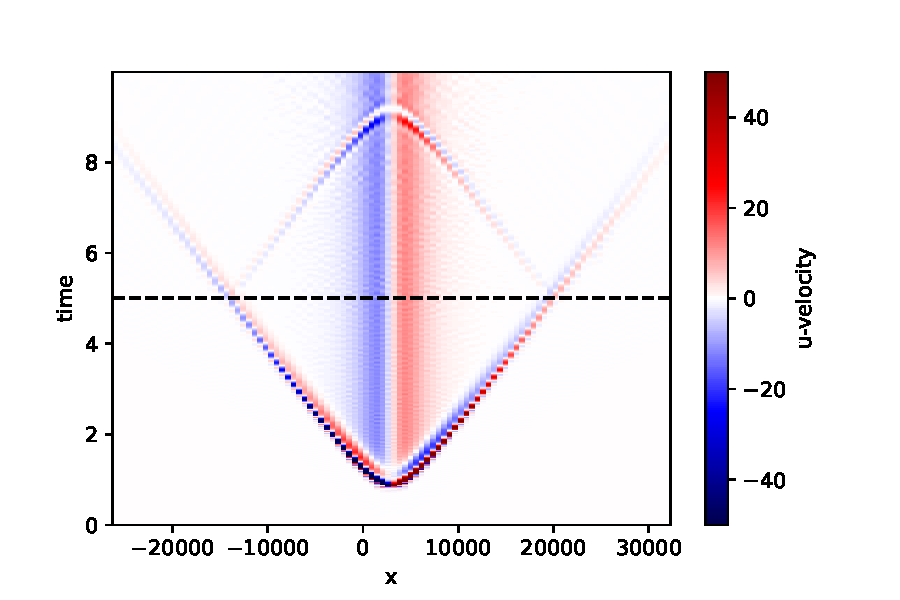
\includegraphics[width=\textwidth]{figures/AcousticITM.pdf}
    \caption{Wave produced by velocity impulse in acoustic media with \ac{ITM}}
\end{subfigure}
\hfill
\begin{subfigure}[t]{0.49\textwidth}
    \centering 
    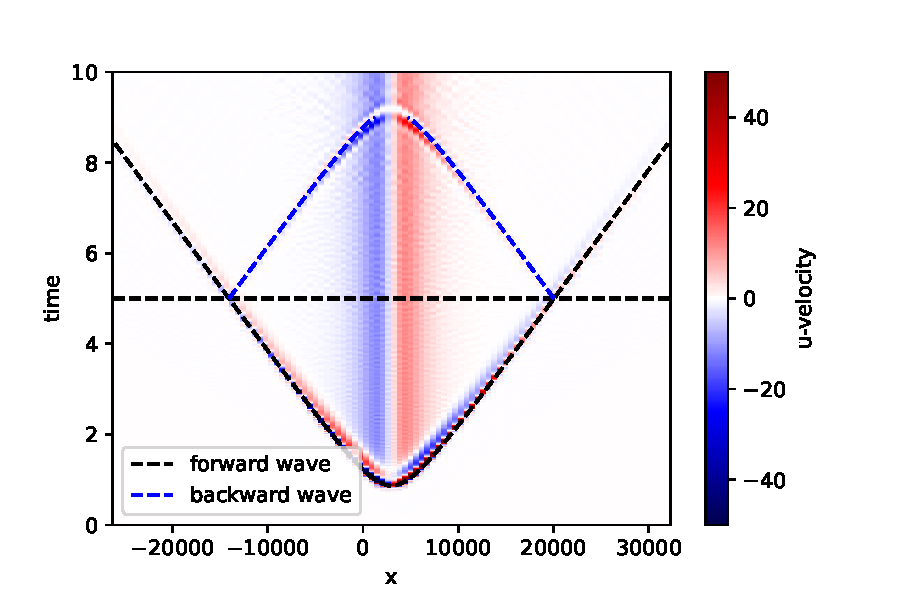
\includegraphics[width=\textwidth]{figures/AcousticITMAnnotated.pdf}
    \caption{Expected location of forward and reflected waves in time. The dashed lines denote the expected location of the wavefronts at given time.}
    \label{subfig:acousticITMAnnotated}
\end{subfigure}
\caption{Space-time plot for wave produced by velocity impulse point source in acoustic media with \ac{ITM}. We take a slice at $\left(3000,3000,20000\right)$ perpendicular to the $z$-axis
and plot the $u$-velocity along $x$-axis at different times.}
\label{fig:space-timeplot-acousticITM}
\end{figure}

We notice that there is a reflected wave travelling back to the source which leaves our slice around $t=8.5$, showing that the reflected wave
is reflected along the line $t=5.0$, which is our point in time when we applied the \ac{ITM}. In figure \ref{subfig:acousticITMAnnotated}, we plot the expected
location of the wave front from the forward going and reflected waves assuming that they are spherical waves and they have equal speeds but in opposite directions. 
It is clear that the reflected wavefronts coincide with the expected locations of the wavefronts. This confirms our hypothesis that the reflected wave has the same speed
as the forward going wave. This also confirms that the application of \ac{ITM} produces a reflected wave successfully in acoustic media.

\section{Time-reversal of waves created by a velocity impulse point source in elastic media} \label{sec:elasticITM}
Here, we apply a velocity impulse point source like in section \ref{sec:acousticITM} but on an elastic medium. We choose the material parameters from the half-space of the 
benchmark case WP2-LOH1\footnote[1]{https://seissol.readthedocs.io/en/latest/pointsource.html} to make it a homogenous elastic medium. The material parameters 
are characterized by
\begin{align}
    \begin{split}
        \rho &=    2700.0 ,\\
        \mu &=     3.23980992 \cdot 10^{10} ,\\
        \lambda &= 3.24038016 \cdot 10^{10} ,
    \end{split}
\end{align}
which makes the velocities of P- and S-waves to be
\begin{align}
    \begin{split}
        v_p &= 6000.0 ,\\
        v_s &= 3464.0 .
    \end{split}
\end{align}

In this case we extend our computational domain even further to $\left[-104000,128000\right] \times \left[-104000,128000\right] \times \left[0,136000\right]$ and a simulation time of $t=18.0$ with \ac{ITM} applied at $t=9.0$
such that the originating waves do not reflect back from the boundaries at the $x$- and $y$-axis ensuring that reflections due to the \ac{ITM} are clearly noticeable.
Our velocity impulse source is at $\left(12000,12000,68000\right)$, the center of the domain.
We chose to analyse the simulation for a longer time in this scenario such that the S-wave reaches the slice. We choose an unstructured tetrahedral mesh with around 13 million elements similar to the acoustic case. 
We apply a source which has already been discussed in equation \ref{eq:source} and figure \ref{fig:source}.

We pick a slice at $\left(12000,12000,40000\right)$ and visualise the wavefield with velocity in $x$-direction and the displacement along the $x$-axis. With this setup and velocity impulse, 
we see that the velocity in $x$-direction looks like in figure \ref{fig:space-timeplot-elasticnoITM}.

\begin{figure}[htpb]
    \centering
    \includegraphics[width=0.75\linewidth]{figures/noITMElasticvelocity.pdf}
    \caption{Space-time plot for waves produced by velocity impulse point source in elastic media. We take a slice at $\left(12000,12000,40000\right)$ perpendicular to the $z$-axis
    and plot the $u$-velocity along $x$-axis at different times.}
    \label{fig:space-timeplot-elasticnoITM}
\end{figure}

We integrate the obtained velocity field to plot displacement field in $x$-direction as shown in figure \ref{fig:space-timeplot-elasticnoITMdisplacement}.

\begin{figure}[htpb]
    \centering
    \includegraphics[width=0.85\linewidth]{figures/noITMElasticdisplacement.pdf}
    \caption{Space-time plot for waves produced by velocity impulse point source in elastic media. We take a slice at $\left(12000,12000,40000\right)$ perpendicular to the $z$-axis
    and plot the displacement in $x$-direction along $x$-axis at different times. We integrate the velocity field to obtain the displacement field.}
    \label{fig:space-timeplot-elasticnoITMdisplacement}
\end{figure}

We can clearly notice two propagating waves as expected as we are dealing with an elastic medium now. We notice a static displacement field in between the two waves.
This is a common phenomenon in displacement fields built with simulation codes in seismic simulations. 
We now apply \ac{ITM} on the same setup at $t=9.0$. The wavefield with the application of the \ac{ITM} looks like in figure \ref{fig:space-timeplot-elasticITM}.

\begin{figure}[htpb]
    \centering
    \includegraphics[width=0.85\linewidth]{figures/Elastic-tworeflections.pdf}
    \caption{Space-time plot for waves produced by velocity impulse point source in elastic media with \ac{ITM}. We take a slice at $\left(12000,12000,40000\right)$ perpendicular to the $z$-axis
    and plot the $u$-velocity along $x$-axis at different times.}
    \label{fig:space-timeplot-elasticITM}
\end{figure}

We notice that there are two clearly reflected waves travelling back to the source. The faster moving wave i.e., P-wave leaves our slice around 
$t=13.0$ which is around 4 seconds after the application of \ac{ITM} which is the time it travelled through the slice just before the application of \ac{ITM}. 
The slower moving wave, i.e., S-wave also has a reflection symmetric about line $t=9.0$. We now plot the displacement plot in x-direction on the 
slice just like we did in figure \ref{fig:space-timeplot-elasticnoITMdisplacement} in figure \ref{fig:space-timeplot-elasticITMdisplacement}.

\begin{figure}[htpb]
    \centering
    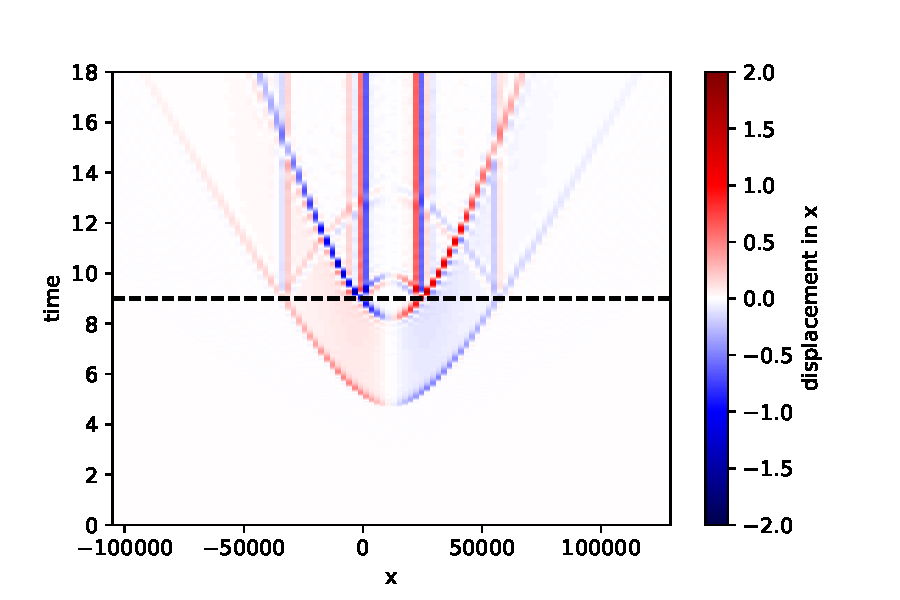
\includegraphics[width=0.75\linewidth]{figures/Elastic-tworeflections-displacement.pdf}
    \caption{Space-time plot for waves produced by velocity impulse point source in elastic media with \ac{ITM}. We take a slice at $\left(12000,12000,40000\right)$ perpendicular to the $z$-axis
    and plot the displacement in $x$-direction along the $x$-axis at different times. We integrate the velocity field to obtain the displacement field.}
    \label{fig:space-timeplot-elasticITMdisplacement}
\end{figure}

We see two reflections even in case of the displacement wavefield too and the static displacements between the two waves persist. But we see extra features here in case of the displacement wavefield. We obtain extra static displacements in time as vertical streaks which originate from the point where the waves meet the slice at \ac{ITM}. These are not yet explained but we suspect they may be explained either by the physical phemonenon or due to the numerical implementation or due to errors produced to numerical integration of the velocity wavefields.
\par This shows that both the waves can be reflected simultaneously by scaling the material parameters to change their impedance to obtain a component which 
is reflected back to its source.

\section{Time-reversal of P-wave created by a velocity impulse point source in elastic media} \label{sec:elasticITMpwave}
We now demonstrate the reflection of just the P-wave by scaling the Lam\'{e} parameter $\lambda$ and keeping the second Lam\'{e} parameter $\mu$ constant.
\par The same setup is used as in section \ref{sec:elasticITM} and we try to reflect just the P-wave while letting the S-wave travel unaffected in time. The slice
and everything else about the simulation setup remain the same. The wavefields without \ac{ITM} are given in figures \ref{fig:space-timeplot-elasticnoITM} and
\ref{fig:space-timeplot-elasticnoITMdisplacement}
\par After the application of the \ac{ITM}, we see a reflection in the wavefield in figure \ref{fig:space-timeplot-pwave}.
As the reflection in figure \ref{fig:space-timeplot-pwave} is visible but is faint, we plot the same with a different colorbar just to show the reflection in a clearer
way as depicted in figure \ref{fig:space-timeplot-pwave2}
\begin{figure}[htpb]
    \centering
    \includegraphics[width=0.75\linewidth]{figures/pwave-ITM1.pdf}
    \caption{Reflection of P-wave in elastic Media with \ac{ITM}. We take a slice at $\left(12000,12000,40000\right)$ perpendicular to the $z$-axis
    and plot the $u$-velocity along the $x$-axis at different times.}
    \label{fig:space-timeplot-pwave}
\end{figure}

\begin{figure}[htpb] %% replace pictures. Not clear and being cut
    \centering
    \includegraphics[width=0.75\linewidth]{figures/pwave-ITM2.pdf}
    \caption{Reflection of P-wave in elastic media with \ac{ITM}. We take a slice at $\left(12000,12000,40000\right)$ perpendicular to the $z$-axis
    and plot the $u$-velocity along the $x$-axis at different times. We use a different colorbar from figure \ref{fig:space-timeplot-pwave} to show the reflection more clearly.}
    \label{fig:space-timeplot-pwave2}
\end{figure}
\par We can clearly see here in this plot that there is a P-wave which is reflected without affecting the S-wave. This provides us a proof of concept where we 
can reflect one wave by changing its impedance while maintaining the other wave's impedance constant.

\begin{figure}[htpb] %% replace pictures. Not clear and being cut
    \centering
    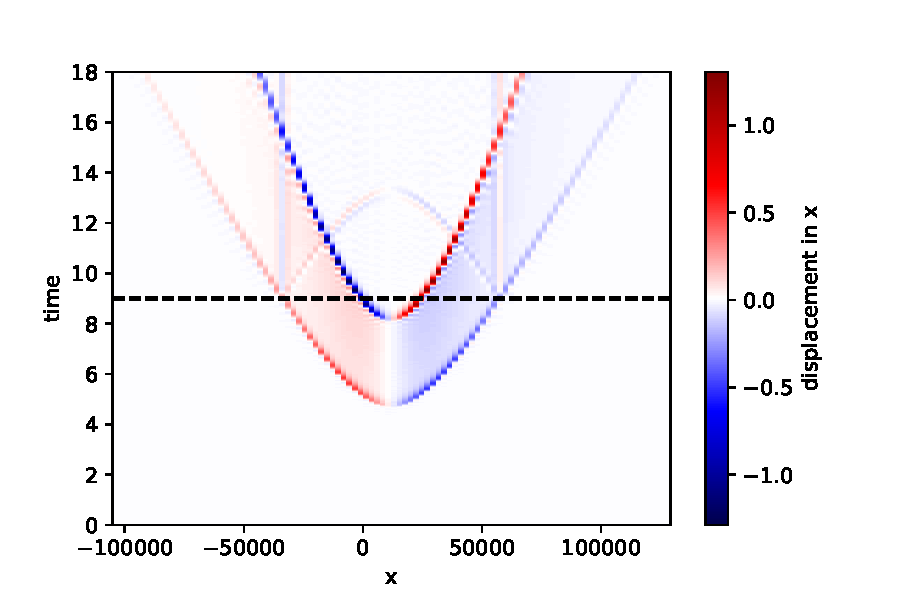
\includegraphics[width=0.75\linewidth]{figures/pwave-ITMdisplacement.pdf}
    \caption{Reflection of P-wave in elastic media with \ac{ITM}. We take a slice at $\left(12000,12000,40000\right)$ perpendicular to the $z$-axis
    and plot the displacement in $x$-direction along the $x$-axis at different times. We integrate the velocity field to obtain the displacement field.}
    \label{fig:space-timeplot-pwavedisplacement}
\end{figure}

We plot the displacement wavefield in figure \ref{fig:space-timeplot-pwavedisplacement} and we can see the reflected P-wave in displacement wavefield and the static
displacement is noticed in this case too just like in the case of reflecting both the waves. 

\section{Time-reversal of S-wave created by a velocity impulse point source in elastic media} \label{sec:elasticITMswave}
In this section, we demonstrate the reflection of just the S-wave by modifying the Lam\'{e} parameters such that P-wave does not
get reflected but the S-wave does. The same setup is used as in section \ref{sec:elasticITM}. The wavefields without \ac{ITM} are given in figures in \ref{fig:space-timeplot-elasticnoITM}
and \ref{fig:space-timeplot-elasticnoITMdisplacement}.
\par After the application of the \ac{ITM}, we see reflections in the wavefield in figure \ref{fig:space-timeplot-swave} showing the zoomed version near the 
\ac{ITM} so that the reflected part is clearly visible in figure \ref{subfig:swavezoomed}.

\begin{figure}[htpb]
    \begin{subfigure}[t]{0.49\textwidth}   
        \centering 
        \includegraphics[width=1.2\textwidth]{figures/swaveITM1.pdf}
        \caption{Reflecting S-wave in elastic media. We take a slice at $\left(12000,12000,40000\right)$ perpendicular to the $z$-axis
        and plot the $u$-velocity along the $x$-axis at different times.}
        \label{subfig:swave}
    \end{subfigure}
    \hfill
    \begin{subfigure}[t]{0.49\textwidth}   
        \centering 
        \includegraphics[width=1.2\textwidth]{figures/swaveITM2.pdf}
        \caption{Zoomed cut section of figure \ref{subfig:swave} to show the reflected S-wave more clearly.}
        \label{subfig:swavezoomed}
    \end{subfigure}
    \caption{Reflection of S-wave in elastic media with \ac{ITM}. We take a slice at $\left(12000,12000,40000\right)$ perpendicular to the $z$-axis and plot the $u$-velocity along the $x$-axis at different times.}
    \label{fig:space-timeplot-swave}
\end{figure}
    
We plot the displacement wavefield in figure \ref{fig:space-timeplot-swavedisplacement} and we can see the reflected S-wave in displacement 
wavefield and the static displacement like in previous section persists. We need more investigation into this to understand this static displacement.

\begin{figure}[htpb]
    \centering
    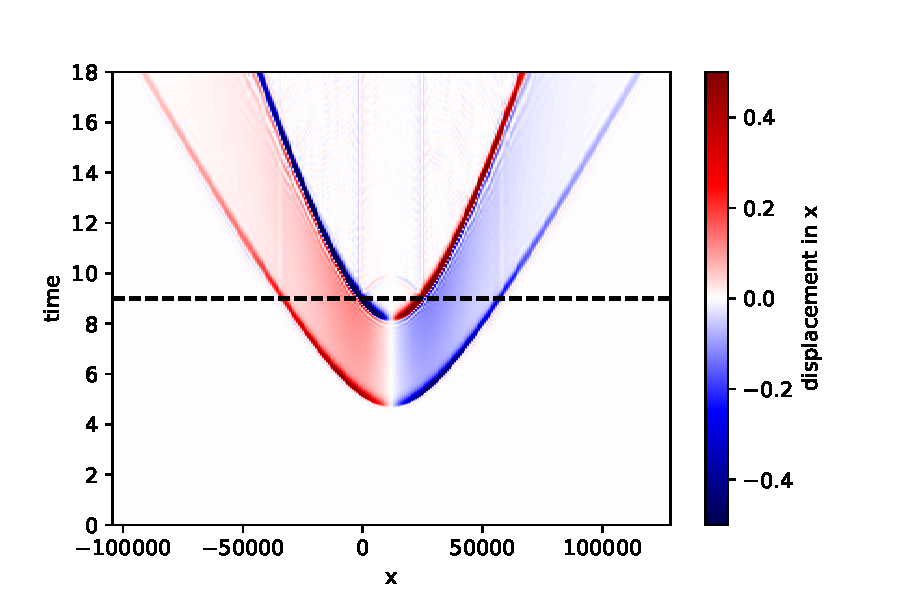
\includegraphics[width=0.85\linewidth]{figures/swaveITMdisplacement.pdf}
    \caption{Reflection of S-wave in elastic media with \ac{ITM}. We take a slice at $\left(12000,12000,40000\right)$ perpendicular to the $z$-axis
    and plot the displacement in $x$-direction along the $x$-axis at different times. We integrate the velocity field numerically to obtain the displacement field.}
    \label{fig:space-timeplot-swavedisplacement}
\end{figure}

We see here in figure \ref{fig:space-timeplot-swave} that there is a S-wave which is reflected without affecting the P-wave. 
This provides us a proof of concept where we show that we can reflect one wave by changing its impedance while maintaining the other wave's impedance constant.

\section{Time-reversal of wave created by a pressure impulse point source in acoustic media}\label{sec:pressureimpulse}
We choose the same material and mesh as in section \ref{sec:acousticITM} and change the source term to a pressure impulse. A pressure impulse source term is a moment tensor
with all non-diagonal elements zero and equal diagonal elements~\parencite[Cha. 9]{shearer_2019}. These are applied to the first three equations of the set of equations \ref{eq:setofequations}. 
An exponentially decaying source is chosen similar to the source in section \ref{sec:acousticITM}. With this setup, the normal propagation of the wave looks at a slice which is already explained in section \ref{sec:acousticITM}
like in figure \ref{fig:space-timeplot-pressurenoITM}.

\begin{figure}[htpb]
    \centering
    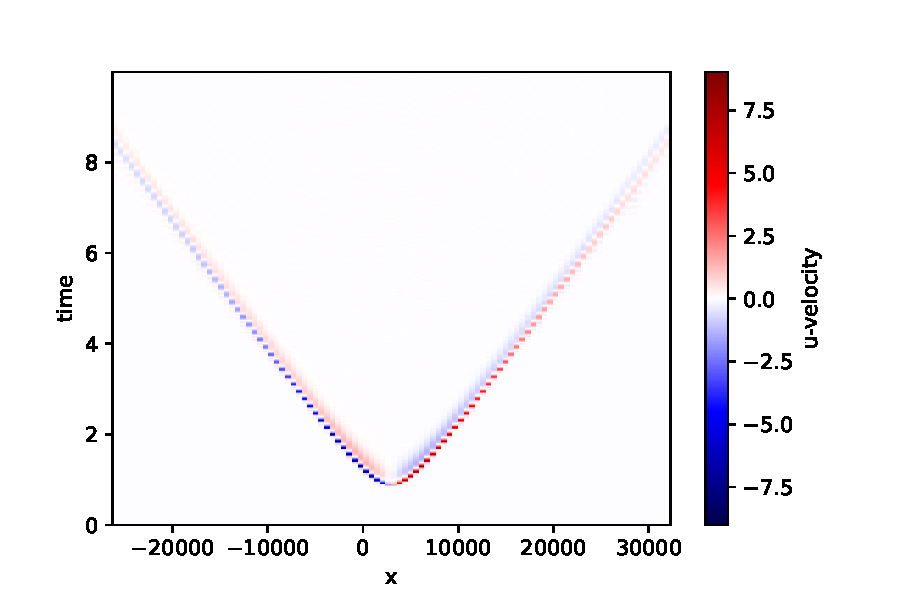
\includegraphics[width=0.75\linewidth]{figures/pressureimpulsewave-noITM.pdf}
    \caption{Space-time plot for wave produced by pressure impulse point source in acoustic media. We take a slice at $\left(3000,3000,20000\right)$ perpendicular to the $z$-axis and plot the
    $u$-velocity along the $x$-axis at different times.}
    \label{fig:space-timeplot-pressurenoITM}
\end{figure}

We notice that we have only one wave propagating in time as expected as we have an acoustic medium and it reaches our slice around $t=1.5$. We now apply \ac{ITM} at $t=5.0$ and the wavefield looks like in figure \ref{fig:space-timeplot-pressureITM}.

\begin{figure}[htpb]
    \centering
    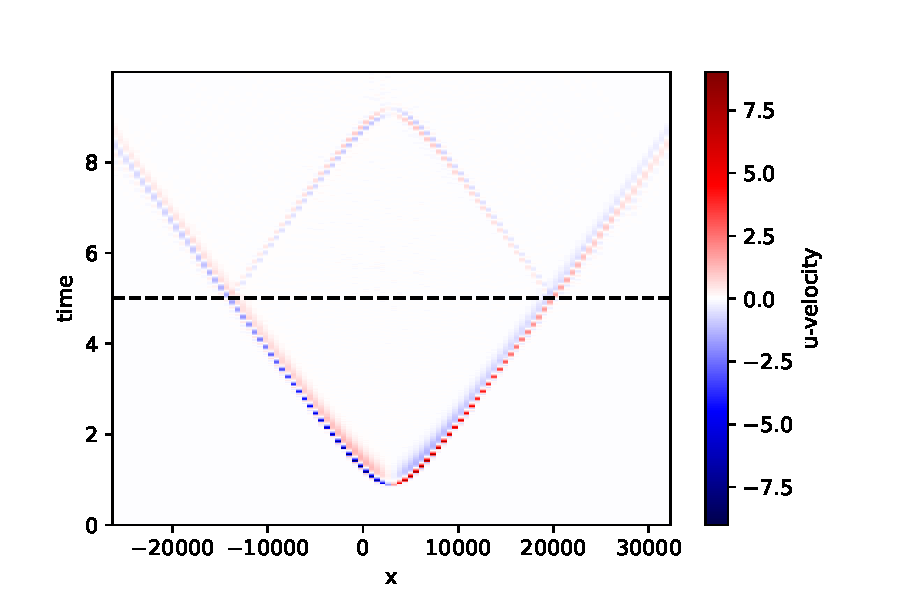
\includegraphics[width=0.75\linewidth]{figures/pressure-impulse-ITM.pdf}
    \caption{Space-time plot for wave produced by pressure impulse point source in acoustic media with \ac{ITM}. We take a slice at $\left(3000,3000,20000\right)$perpendicular to the $z$-axis and plot the
    $u$-velocity along the $x$-axis at different times.}
    \label{fig:space-timeplot-pressureITM}
\end{figure}

We notice that there is a reflected wave travelling back to the source. The reflected wave leaves our slice around $t=8.5$, showing that the reflected wave is reflected
along the line $t=5.0$, which is our point in time when we applied the \ac{ITM}. This confirms that the application of \ac{ITM} produces a reflected wave successfully in acoustic media even
when the waves are created by pressure impulse point sources.

\section{Time-reversal of waves created by a force couple moment tensor in elastic media}\label{sec:doublecouple}
We now apply a force couple moment tensor as a source term in an elastic medium.~\parencite[Sec. 9.2]{shearer_2019} defines a force couple moment tensor as

\begin{align}
    \begin{split}
        \mathbf{M} =
            \begin{bmatrix}
                M_{11} & M_{12} & M_{13} \\
                M_{21} & M_{22} & M_{23} \\
                M_{31} & M_{32} & M_{33} \\
            \end{bmatrix} ,
    \end{split}
\end{align}

where $M_{ij}$ is a pair of opposing forces pointing in $i$-direction, separated in the $j$-direction. The condition that angular momentum is conserved requires that $M_{ij} = M_{ji}$. As a consequence, $\mathbf{M}$ has only six independent elements. The moment tensor is applied to the first six equations of the set of equations \ref{eq:setofequations} as per the direction it is to be applied~\parencite{10.1785/0120060253}.
\subsection{Moment tensor with non-diagonal elements zero}
We begin with a moment tensor which has only diagonal elements not equal to each other. The material parameters and simulation setup are the same as in section \ref{sec:elasticITM}. The moment tensor chosen is

\begin{align}
    \begin{split}
        \mathbf{M} =
            \begin{bmatrix}
                0.9 & 0.0 &0.0 \\
                0.0 & 0.1 & 0.0 \\
                0.0 & 0.0 & -0.1 \\
            \end{bmatrix} \times 10^{19} .
    \end{split}
\end{align}

With this setup, the space-time plot at the slice chosen looks as shown in figure \ref{fig:space-timeplot-doublecouplediagnoITM}.

\begin{figure}[htpb]
    \centering
    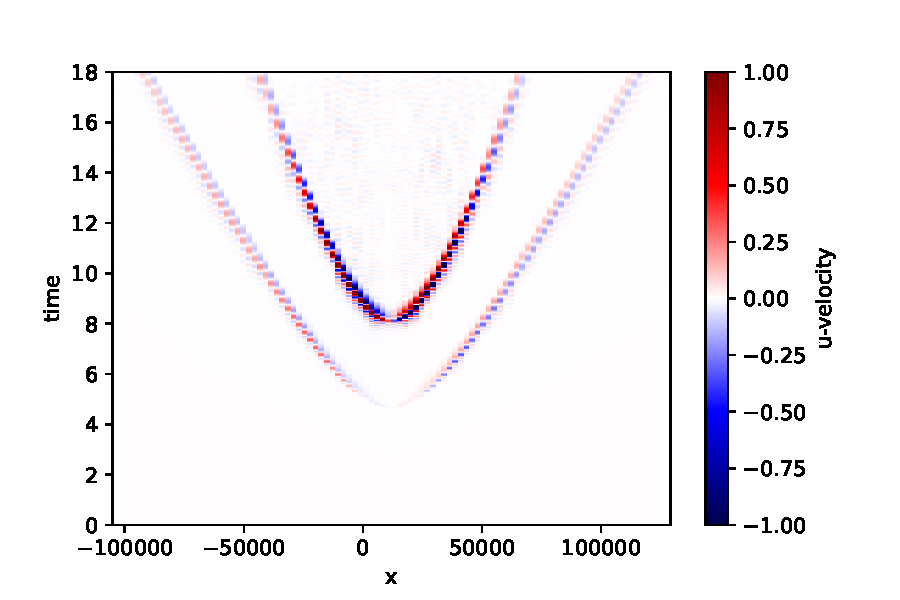
\includegraphics[width=0.75\linewidth]{figures/double-couple-diag-noITM.pdf}
    \caption{Space-time plot for waves produced by force couple moment tensor with non-diagonal elements zero in elastic media. We take a slice at $\left(12000,12000,40000\right)$ perpendicular to the $z$-axis and plot the $u$-velocity along the $x$-axis at different times.}
    \label{fig:space-timeplot-doublecouplediagnoITM}
\end{figure}

We now apply \ac{ITM} at $t=9.0$ and notice that both the waves are reflected as expected in figure \ref{fig:space-timeplot-doublecouplediagITM}.

\begin{figure}[htpb]
    \centering
    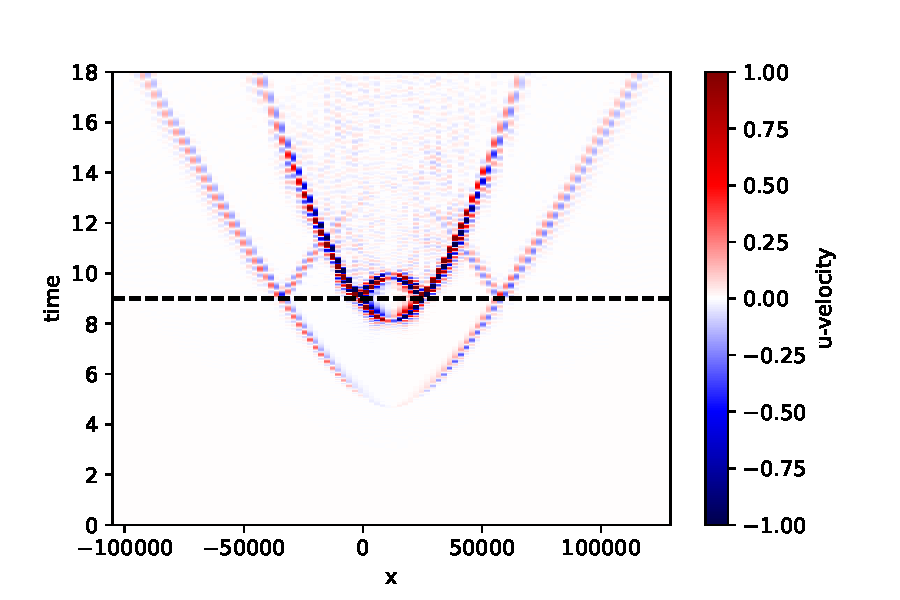
\includegraphics[width=0.8\linewidth]{figures/double-couple-diag.pdf}
    \caption{Space-time plot for waves produced by force couple moment tensor with non-diagonal elements zero in elastic media with \ac{ITM}. We take a slice at $\left(12000,12000,40000\right)$ perpendicular to the $z$-axis and plot the $u$-velocity along the $x$-axis at different times.}
    \label{fig:space-timeplot-doublecouplediagITM}
\end{figure}
As expected, there are two reflections in the wavefield. This confirms that \ac{ITM} could be used to obtain a reversed wave in case of waves generated by a force couple moment tensor.

\subsection{Moment tensor with non-diagonal elements non-zero}
We now use a moment tensor obtained from a seismic event that occured near Tori Shima, Japan~\parencite{kanamori},~\parencite{shearer_2019}. 
To obtain stable results, the isotropic component is constrained to zero as

\begin{align}
    \begin{split}
        \mathbf{M} =
            \begin{bmatrix}
                -1.8 & -0.38 & -0.96 \\
                -0.38 & -1.9 & 0.62 \\
                -0.96 & 0.62 & 3.7 \\
            \end{bmatrix} \times 10^{17} .
    \end{split}
\end{align}

With this setup, the space-time plot at the slice chosen looks as shown in figure \ref{fig:space-timeplot-doublecoupletorinoITM}.

\begin{figure}[htpb]
    \centering
    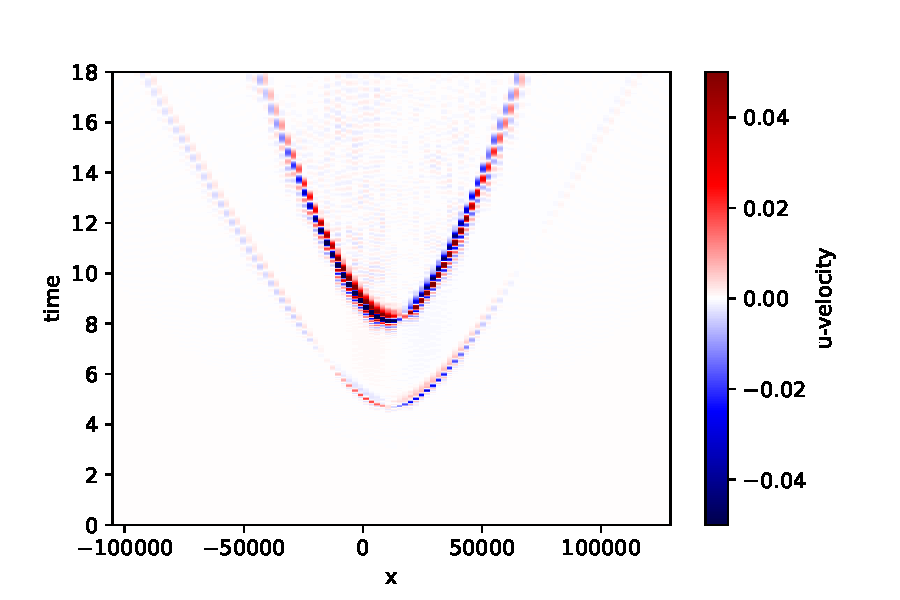
\includegraphics[width=0.8\linewidth]{figures/double-couple-tori-noITM.pdf}
    \caption{Space-time plot for waves produced by force couple moment tensor with non-diagonal elements in elastic media. We take a slice at $\left(12000,12000,40000\right)$ perpendicular to the $z$-axis and plot the $u$-velocity along the $x$-axis at different times.}
    \label{fig:space-timeplot-doublecoupletorinoITM}
\end{figure}

We now apply \ac{ITM} at $t=9.0$ and notice that both the waves are reflected as expected in figure \ref{fig:space-timeplot-doublecoupletoriITM}.

\begin{figure}[htpb]
    \centering
    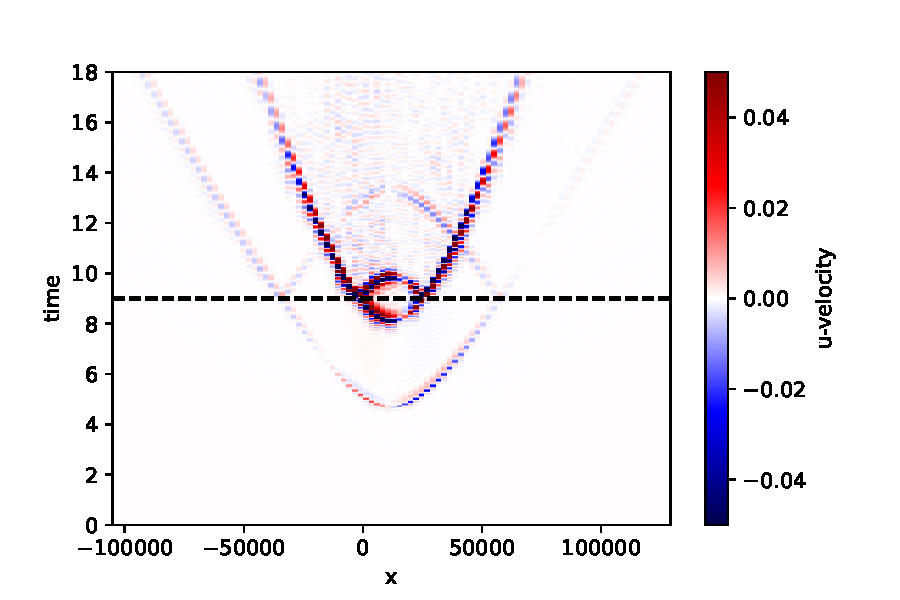
\includegraphics[width=0.75\linewidth]{figures/double-couple-tori2.pdf}
    \caption{Space-time plot for waves produced by force couple moment tensor with non-diagonal elements in elastic media with \ac{ITM}. We take a slice at $\left(12000,12000,40000\right)$ perpendicular to the $z$-axis and plot the $u$-velocity along the $x$-axis at different times.}
    \label{fig:space-timeplot-doublecoupletoriITM}
\end{figure}

As expected, there are two reflections in the wavefield. This confirms that \ac{ITM} could be used to obtain a reversed wave in case of waves generated by a force couple moment tensor even when there are non-zero non diagonal elements.
\section{Convergence Test}\label{sec:convergence}
We now perform a convergence test to verify that our \ac{ITM} implementation is accurate and converges with our \ac{ADER}-\ac{DG} scheme. 
We check the error between our numerical implementation and the analytical solution developed in section \ref{section:3DITMAcoustic}. 
The mesh is setup with equal triangular elements on a cubic domain of $\left[-1, 1\right] \times \left[-1, 1\right] \times \left[-1, 1\right]$ with the number of elements in each direction varying in $\left[4, 8, 16, 32, 64, 128\right]$.
We calculate the $L^2$ error of $u$-velocity of the solution with respect to the analytical solution as per section \ref{section:3DITMAcoustic}. We calculate this error for different polynomial
orders within $\left[1, 2, 3, 4, 5\right]$ used in the reference element of the \ac{DG} scheme. We expect a convergence order of $p+1$ where $p$ is the polynomial order used in the
\ac{DG} scheme used ~\parencite{cockburn2011discontinuous}. We now plot the $L^2$ error norm of $u$-velocity in figure \ref{fig:convergence}.

\begin{figure}[htpb]
    \centering
    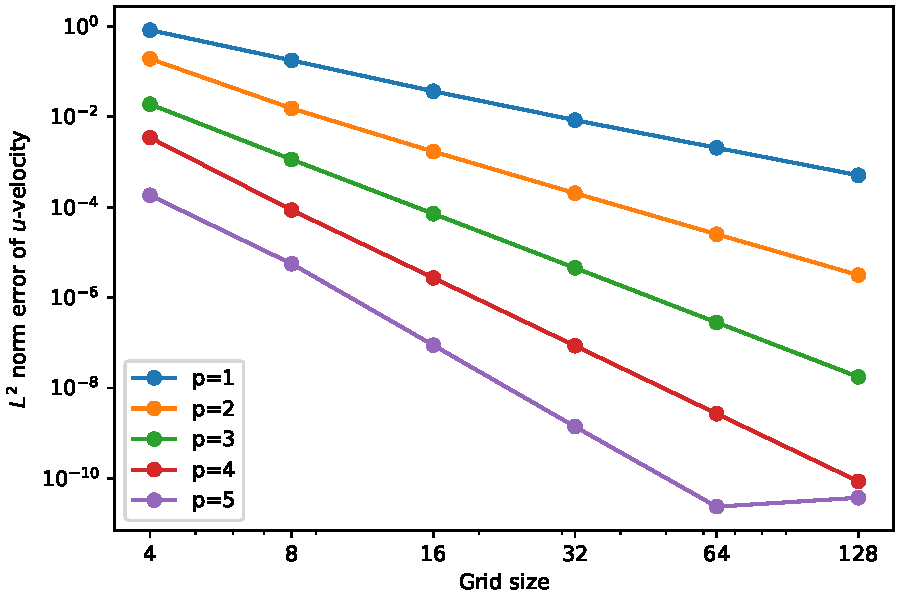
\includegraphics[width=0.8\linewidth]{figures/error1.pdf}
    \caption{Convergence plot for $L^2$ norm of $u$-velocity for acoustic travelling wave with \ac{ITM}. The error is calculated with respect to the analytical solution
    in section \ref{section:3DITMAcoustic}.}
    \label{fig:convergence}
\end{figure}

We notice that the slope of the curve increases as expected with increasing order of the polynomial. In case of order 5, there is a slight increase
of error for grid size 128. This is suspected to be due to the error plateauing as the precision hits the floating point precision. We perform a linear fit on the log-log
plot to get a slope such that we can check the convergence order of the plot. We remove the last point from the fit for $p=5$ as it is suspected to be an outlier. 
We get the following convergence orders for different polynomial orders shown in table \ref{table:convergenceorder} and figure \ref{fig:convergenceorder}.

\begin{center}
\begin{table}[htpb]
    \centering
    \caption{Convergence order vs polynomial order obtained from the convergence study of acoustic travelling wave with \ac{ITM}}.
    \label{table:convergenceorder}
    \begin{tabular}{|l|l|}
        \hline
     \textbf{Polynomial Order}& \textbf{Convergence Order}  \\
     \hline
     1 & 2.13\\
     \hline
     2 & 3.15 \\
     \hline
     3 & 4.00 \\
     \hline
     4 & 5.03 \\
        \hline
        5 & 5.77\\
        \hline
    \end{tabular}
    \end{table}
\end{center}
We now plot the expected error with the expected convergence order vs the actual error during the simulations in figure \ref{fig:expectedvsactualerror}.
\begin{figure}[htpb]
    \centering
    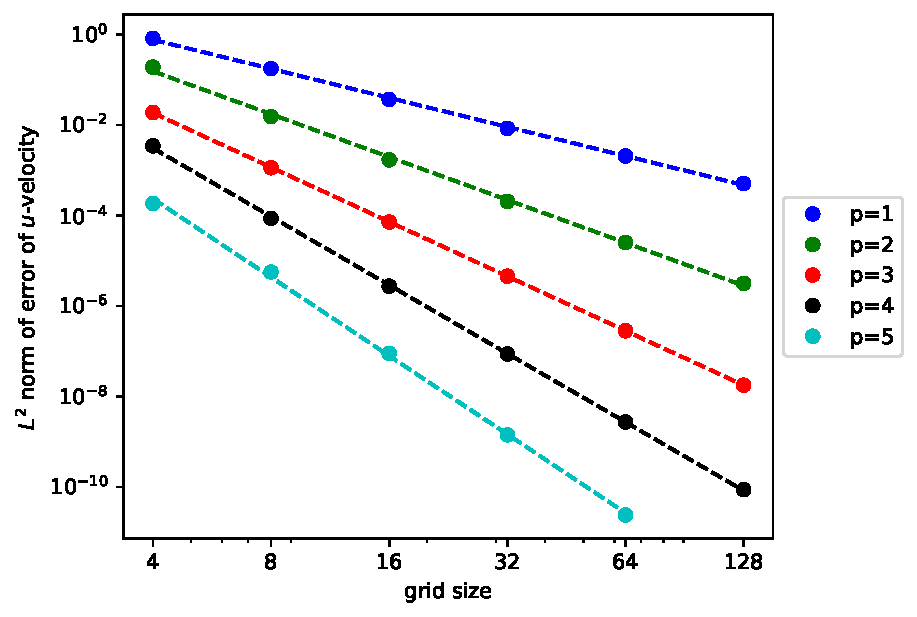
\includegraphics[width=0.75\linewidth]{figures/error2.pdf}
    \caption{Linear fit of $\log\left(L^2\right)$ and $\log\left(grid size\right)$  plot for acoustic travelling wave with \ac{ITM}. Dashed lines denote the linear fit of the logarithms. The slope of the dashed lines denotes the obtained convergence order. The outlier for $p=5$ is removed from the fit.}
    \label{fig:convergenceorder}
\end{figure}
\begin{figure}[htpb]
    \centering
    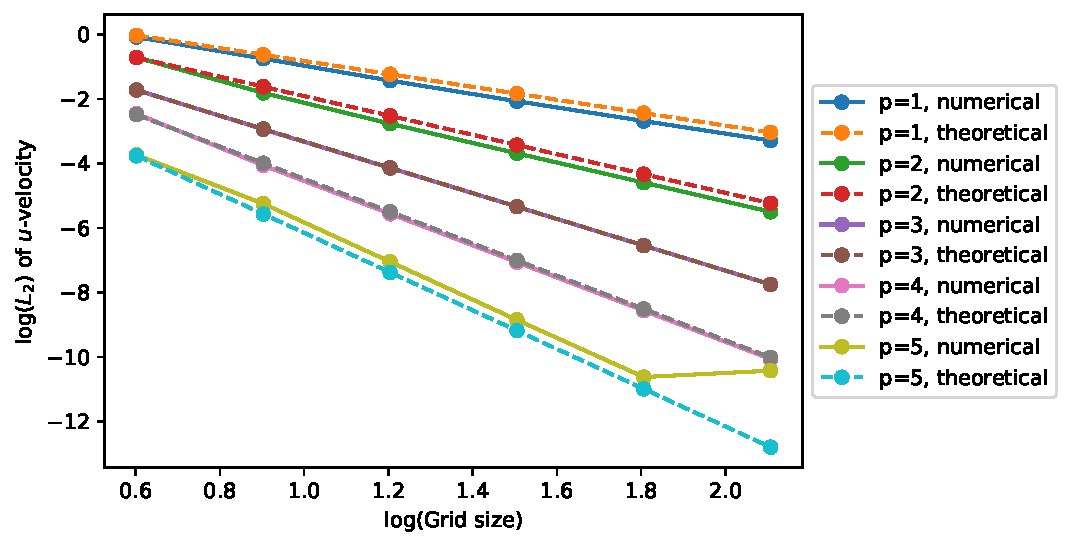
\includegraphics[width=0.75\linewidth]{figures/error3.pdf}
    \caption{Expected $L^2$ norm vs actual $L^2$ norm for acoustic travelling wave with \ac{ITM}. Solid lines denote the original error where as the dashed lines are the expected error. The expected error is calculated with the expected convergence order
    as the slope and the mean of logarithms of errors as the intercept of the line.}
    \label{fig:expectedvsactualerror}
\end{figure}

We notice that our numerical error agrees with the expected theoretical error well. This concludes the correctness of our implementation of \ac{ITM} in SeisSol with \ac{ADER}-\ac{DG}.

\section{Discussion}
In this chapter, we looked at the results obtained from applying the \ac{ITM} on seismic waves. We began with the reflection of a travelling planar wave in acoustic media
and then moved on to spherical waves generated by a velocity impulse point source in acoustic and elastic media. 
We then looked at the reflection of just the P-wave and S-wave separately to show that we can reflect just one wave by changing its impedance while keeping the other wave's impedance constant.
In the end, we ran a convergence study of our implementation with the analytical solution obtain in section \ref{section:3DITMAcoustic} to conclude that our implementation
is convergent with the expected convergence order. \\